% Polished boss note: OOD + alignment → category-shift adapt.
% Compile from docs/method/: pdflatex Feature_vs_sample_weights.tex
\documentclass[11pt]{article}
\usepackage[margin=1in]{geometry}
\usepackage{amsmath,amssymb,booktabs,hyperref,array,graphicx,caption}
\usepackage[T1]{fontenc}
\usepackage{lmodern}

\title{OOD $+$ Alignment $\to$ Category-Shift Adaptation\\
\large A cheap \texttt{partial\_fit} recipe for new-category cold-start}
\author{AS-DTA / CFPerm}
\date{}

\begin{document}
\maketitle

\begin{abstract}
\noindent
\textbf{One-liner.}
Quantify category shift as OOD, then adapt a CE head with three cheap
weights via \texttt{partial\_fit}: feature (VIMP), sample (membership),
alignment (hop/prototype cosine). Soft$^{\gamma=0.5}$ tapers empowerment
by $200$ samples/category. The polished online recipe is
\textbf{recommended}: \texttt{both$+$align} while the new category is
scarce, then \texttt{both}.
On text multiclass (FULL LIVE holdout), recommended lifts early acc
($0.456\to\mathbf{0.481}$ at $20$/cat) and finishes at
$\mathbf{+0.014}$ overall vs uniform.
\end{abstract}

%======================================================================
\section{Recipe (what to ship)}
%======================================================================

\begin{center}
\small
\begin{tabular}{@{}llp{7.2cm}@{}}
\toprule
Step & Object & Role \\
\midrule
1. Quantify
  & RF-domain VIMP $v$, membership $m$
  & Where LIVE differs from REF \\
2. Align
  & $\mathrm{align}=\sigma(\beta(\cos_{\mathrm{nov}}-\cos_{\mathrm{known}}))$
  & High alignment with novel direction $\to$ upweight \\
3. Adapt
  & feature / sample / align $\to$ \texttt{sample\_weight}
  & CE \texttt{partial\_fit} only \\
4. Gate
  & soft$^{\gamma=0.5}$, $N_{\mathrm{cap}}=200$
  & Empower, then taper --- no EWMA \\
\bottomrule
\end{tabular}
\end{center}

\paragraph{Recommended online policy.}
\begin{equation*}
  \texttt{recommended}
  =
  \begin{cases}
    \texttt{both$+$align}
      & \text{if cold-start frac }\ge 0.75,\\
    \texttt{both}
      & \text{otherwise.}
  \end{cases}
\end{equation*}
Use alignment when the new category is scarce; drop it once most novel
mass is past the cap. Still one linear head.

%======================================================================
\section{Evidence (FULL LIVE holdout)}
%======================================================================

\begin{figure}[htbp]
\centering
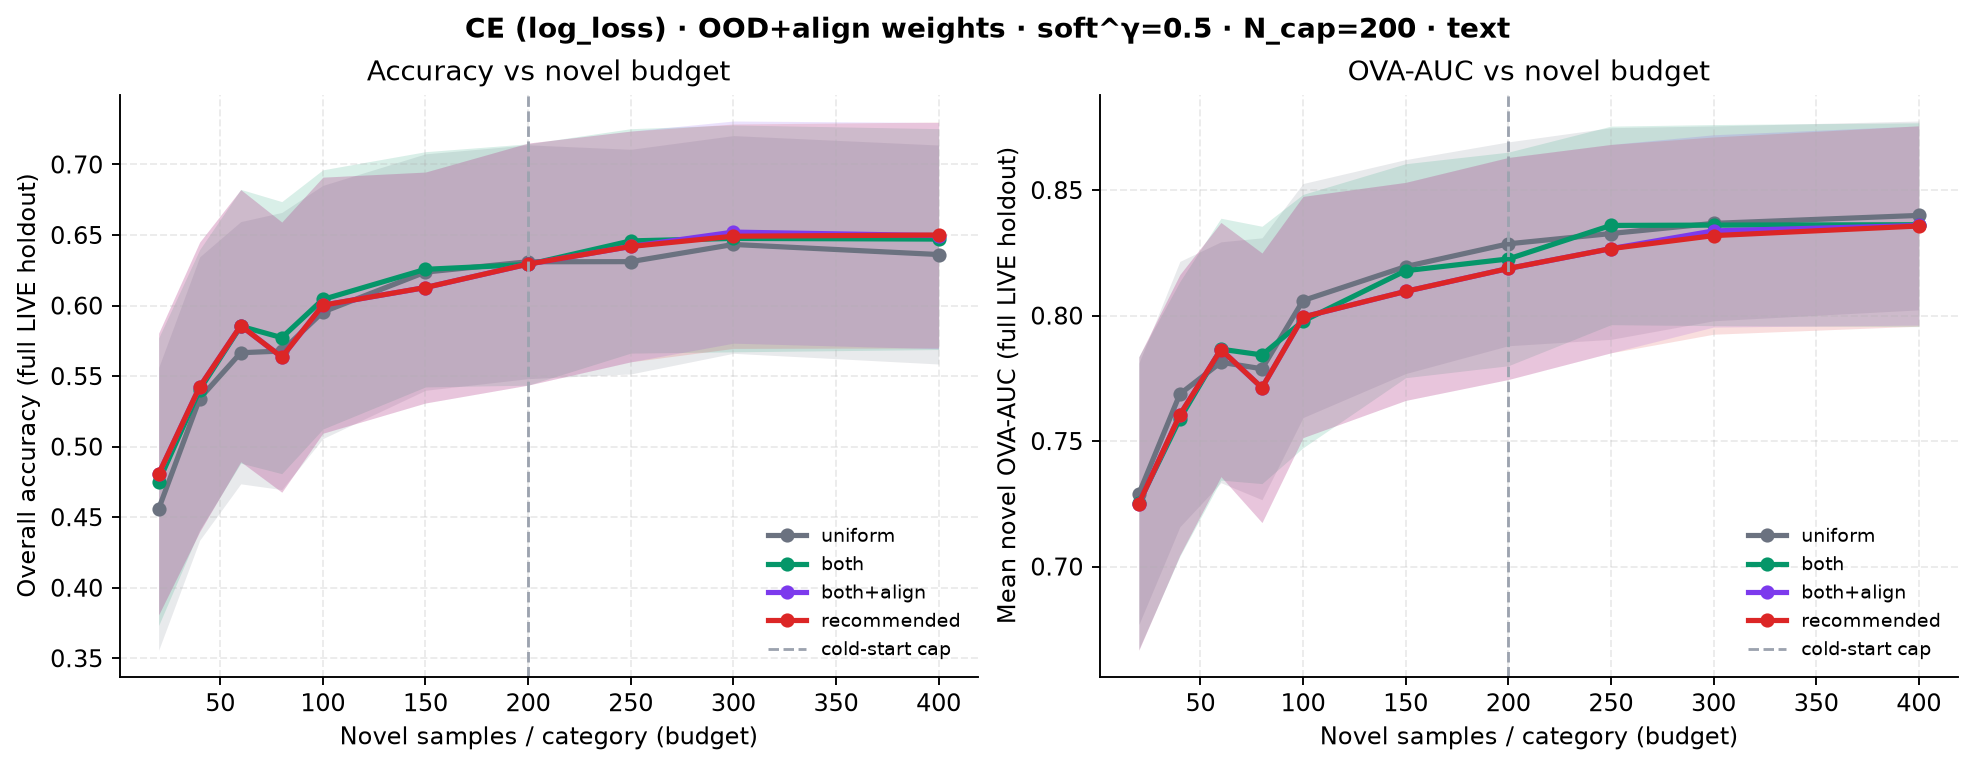
\includegraphics[width=\textwidth]{text_full_weight_acc_auc_curves.png}
\caption{Polished comparison (mean$\pm$SEM): uniform, both,
both$+$align, recommended.
Dashed line: $N_{\mathrm{cap}}=200$.
Recommended tracks both$+$align early and stays on top late.}
\label{fig:curves}
\end{figure}

\begin{figure}[htbp]
\centering
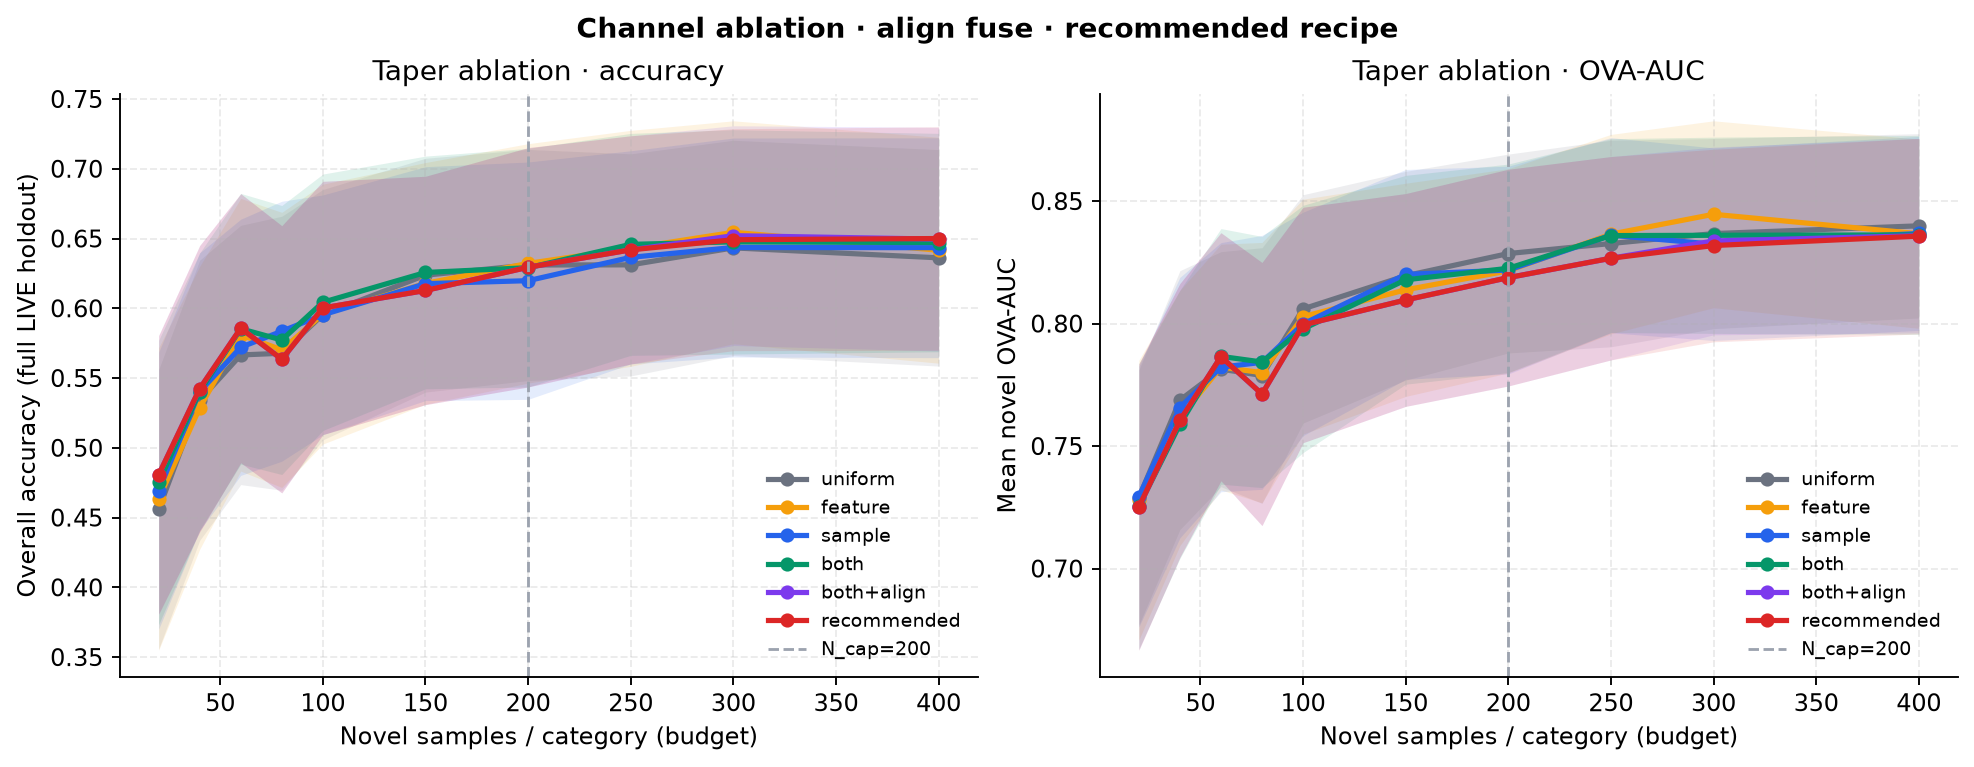
\includegraphics[width=\textwidth]{text_full_weight_gate_ablation.png}
\caption{Channel ablation. Feature / sample / both / align / recommended.
Recommended is the ship default.}
\label{fig:ablate}
\end{figure}

\begin{center}
\small
\begin{tabular}{@{}lcccc@{}}
\toprule
 & uniform & both & both$+$align & \textbf{recommended} \\
\midrule
acc @ $b{=}20$/cat
  & $0.456$ & $0.475$ & $\mathbf{0.481}$ & $\mathbf{0.481}$ \\
endpoint acc
  & $0.636$ & $0.647$ & $0.650$ & $\mathbf{0.650}$ \\
endpoint $\Delta$acc
  & --- & $+0.011$ & $+0.013$ & $\mathbf{+0.014}$ \\
\bottomrule
\end{tabular}
\end{center}

\paragraph{Cost.}
One shallow RF $+$ a few CE \texttt{partial\_fit} epochs.
No new backbone, no EWMA schedule.

%======================================================================
\section{Takeaway}
%======================================================================

\begin{enumerate}
  \item Category shift $=$ OOD; quantify once, adapt with weights.
  \item Alignment is the same ``high align $\to$ upweight'' family as
        hop-cosine IW --- plug into \texttt{sample\_weight}.
  \item Ship \textbf{recommended}: align while scarce, then both.
\end{enumerate}

\end{document}
